\documentclass[11pt,a4paper,titlepage,oneside]{book}

\usepackage[czech]{babel}
\usepackage[utf8]{inputenc}
\usepackage{graphicx}
\usepackage{url}
\usepackage{fancyhdr}
\usepackage{setspace}
\usepackage{hyperref}
\usepackage{rotating}


%\usepackage{titlesec}
%\titleformat{\chapter}{\normalfont\LARGE\bfseries}{\thechapter}{1em}{}
%\titlespacing*{\chapter}{0pt}{3.5ex plus 1ex minus .2ex}{2.3ex plus .2ex}


\begin{document}

%nastavení fancy stylu
\lhead{
\includegraphics[height=0.5cm]{obrazky/lev.jpg} {ČVUT v~Praze}}
\rhead{\leftmark}
\cfoot{\thepage}
\setlength{\headheight}{24pt}

\pagestyle{empty}	%%vypne číslování

\begin{titlepage} %% titulní strana 1(bez lva)
	\begin{center}
		{\huge ČESKÉ VYSOKÉ UČENÍ TECHNICKÉ} \\ [0.25cm]
		{\LARGE FAKULTA STAVEBNÍ}
		\\[9cm]		
		{\Huge DIPLOMOVÁ PRÁCE}
		\\[9cm]
		{\Large Praha 2013 \hspace{\stretch{1}} Chrudoš VORLÍČEK}
	\end{center}
\end{titlepage}

\begin{titlepage} %%titulní strana 2 (se lvem)
	\begin{center}
		{\huge ČESKÉ VYSOKÉ UČENÍ TECHNICKÉ} \\
		{\LARGE FAKULTA STAVEBNÍ \\ [0.25cm]OBOR GEOINFORMATIKA}
		\\[1cm]
		\begin{figure}[!h]
		\begin{center}
		
\includegraphics[height=5cm]{obrazky/lev.jpg}
		\\[1cm]
		\end{center}
		\end{figure}							
		{\Huge DIPLOMOVÁ PRÁCE \\ [0.25cm]}
		{\LARGE \uppercase {Prototyp turistického systému zaloŽeného na datech \\[0.25cm] OpenStreetMap}}
		\\[3.5cm]
		{\Large Vedoucí práce: Ing. Martin LANDA, Ph.D. \\[0.25cm] Katedra geomatiky}
		\\[1cm]
		{\Large Praha 2013 \hspace{\stretch{1}} Chrudoš VORLÍČEK}
	\end{center}
\end{titlepage}

\newpage %%zadání
	\begin{center}
		\vspace*{15cm}
		{\Large ZDE VLOŽIT LIST ZADÁNÍ}
	\end{center}

%% Abstrakt
\begin{flushleft}
	\chapter*{}
	\section*{ABSTRAKT}
	\paragraph{} Hlavním tématem této práce je tvorba webové turistické aplikace za použití dat OpenStreetMap, jeho napojení na sociální síť Facebook a přidávání dat přímo do OpenStreetMap. Součástí práce je i stručné shrnutí existujích řešení, popsání užitých technologií a jejich výhod a nevýhod.
	\section*{KLÍČOVÁ SLOVA}
	{\sc{OpenStreetMap, OSM, Turistický systém, Facebook, Nette}}
	\section*{ABSTRACT}
	\paragraph{}
	\section*{KEYWORDS}
	{\sc{}}
\end{flushleft}

\newpage %%Prohlášení
	\vspace*{15cm}
	\section*{\Large PROHLÁŠENÍ}
		\paragraph{}Prohlašuji, že jsem diplomovou práci na téma \uv{Prototyp turistického systému založeného na datech OpenStreetMap} vypracoval samostatně a že veškerou použitou literaturu a podkladové materiály uvádím v~seznamu zdrojů.\\[1cm]
	V~Praze dne ....................... \hspace{\stretch{1}}................................. \\
	\hspace*{\stretch{1}} {(podpis autora)\hspace{0.25cm} }
	
\newpage %%Poděkování
	\vspace*{15cm}
	\section*{\Large PODĚKOVÁNÍ}
	\paragraph{}
		
\renewcommand{\baselinestretch}{1.5} %nastaví mezery
\newpage %%Obsah
\pagestyle{plain}
\pagenumbering{arabic}
\setcounter{page}{5}

	\tableofcontents

\newpage %%Obrázky a tabulky
	\listoffigures
	\listoftables


\newpage %%Samotný text
%%Úvod
\chapter*{Úvod}
\addcontentsline{toc}{chapter}{Úvod}
	\paragraph{} Pro běžného uživatele internetu se různé mapové portály staly součástí zdrojů, ke kterým se obrací v případě, že shání nějaké informace. Od polohy obchodu po vyhledávání cesty na dovolenou. Mapové aplikace jsou běžnou součástí jiných webových aplikací, kde doplňují textové určení místa i vizuální složkou. Dost často se pro tyto účely používají \textit{Mapy.cz} nebo \textit{GoogleMaps}. Oba zmíněné zdroje poskytují API pro snadné a rychlé připojení do aplikace. Vývoj speciální mapy lze pomocí tohoto API také udělat, ovšem poskytuje mnohem méně možností než jiná řešení. 
	\paragraph{} Obdobou \textit{GoogleMaps} jsou \textit{OpenStreetMap}, které jsou vytvářeny komunitou a na rozdíl od \textit{GoogleMaps} poskytují možnost data stáhnout. Tento přístup má své výhody i nevýhody. Na některých místech jsou mapy podrobnější a přesnější než komerční řešení, jinde zas nedosahují takových kvalit. Komerční mapy se udržují v intervalech daných poskytovatelem mapových podkladů. \textit{OpenStreetMap} naproti tomu poskytuje denní verze mapy.
	\paragraph{} Pro potřeby turistů jsou k dispozici různě sofistikované webové aplikace poskytující rozdílné možnosti vyhledávání a užívání map. Každá z těchto aplikací má své přednosti. Součástí práce je i vytvoření výběru existujících aplikací a popsání jejich výhod, nevýhod a použitelnosti pro turistiku. Užitečné prvky aplikací mohou sloužit jako inspirace při tvorbě vlastní aplikace. 
	\paragraph{} Hlavním tématem práce je samotná tvorba turistické mapové aplikace. K jejímu vytvoření bylo použito množství technologií. Ty budou popsány v kapitole \textit{Použité technologie}. Spolu s tím zde budou uvedeny i technologie, jejichž užití bylo zvažováno, ale které nakonec z různých důvodů použity nebyly.
	\paragraph{}Nejobsáhlejší kapitolou je popis toho, co bylo vytvořeno a jak probíhala realizace. Hlavní požadavky, které by měla aplikace splňovat, jsou tyto:
		\begin{itemize}
			\item aplikace je vyvořena nad daty OpenStreetMap,
			\item aplikaci je možno propojit s účtem na sociální síti Facebook,
			\item do aplikace je možno přidávat vlastní trasy a psát k nim informace,
			\item do aplikace se dají vkládat fotky k zájmovým bodům a trasám a
			\item aplikace umožňuje editovat data projektu OpenStreetMap.
		\end{itemize}
	K dalším požadavkům patří:
		\begin{itemize}
			\item přehledné a příjemné uživatelské rozhraní,
			\item vyhledávání objektů a
			\item vyhledávání cest, tzv. routování.
		\end{itemize}
	
	\paragraph{} V závěru práce budou zhodnoceny výsledky tvorby -- co bylo realizováno, co se nepovedlo dokončit a co se nakonec vůbec nevytvářelo. Také zde budou navrženy možnosti dalšího rozšíření.


\pagestyle{fancy}


%%%%%%%%%%%%%%%%%%%%%%%
%%%%% EXISTUJÍCÍ ŘEŠENÍ 	   %%%%%
%%%%						      %%%%
%%%							  %%%
%%								     %%
%									 %
\chapter{Existující řešení}
	\paragraph{} Pro shrnutí, co v současnosti poskytují mapové aplikace, byly zvoleny dvě v České republice nejužívanější aplikace (GoogleMaps a Mapy.cz), aplikace vytvořená pomocí API od Googlu (Výletník) a dvě aplikace postavené na Open StreetMap (Waymarked Trails a OpenTrackMap). Každá z těchto aplikací je něčím specifická, každá má své přednosti i své nedostatky. V této kapitole bude stručně pospáno, jak ta či ona aplikace vyniká a co jí zas chybí.
	\section{Google Mapy}
		\url{http://www.google.com/maps/preview}
		\paragraph{}Google Mapy jsou mapovou aplikací firmy Google. Jejich API je volně k použití, takže ji mnoho jiných aplikací používá. Google mapy neposkytují informace o turistických a cykloturistických stezká. Na druhou stranu mají dobré vyhledávání míst a cest. GoogleMaps též umožňují import vlastních cest. 
		\paragraph{}Důvodem, proč jsou Google mapy začleněné v tomto výběru, je aplikace Panoramio, která umožňuje importovat do mapy fotografie. Ty lze přiřadit k místům a je možné je i komentovat. Ikdyž aplikace Mapy.cz  také poskytují tuto funkcionalitu, je třeba mít na paměti, že Google s ní přišel první.
		\paragraph{}Celkově jsou Google Mapy vhodnější pro navigaci ve městě a na silnicích než v přírodě.

		\begin{figure}[!h]
			\begin{center}
				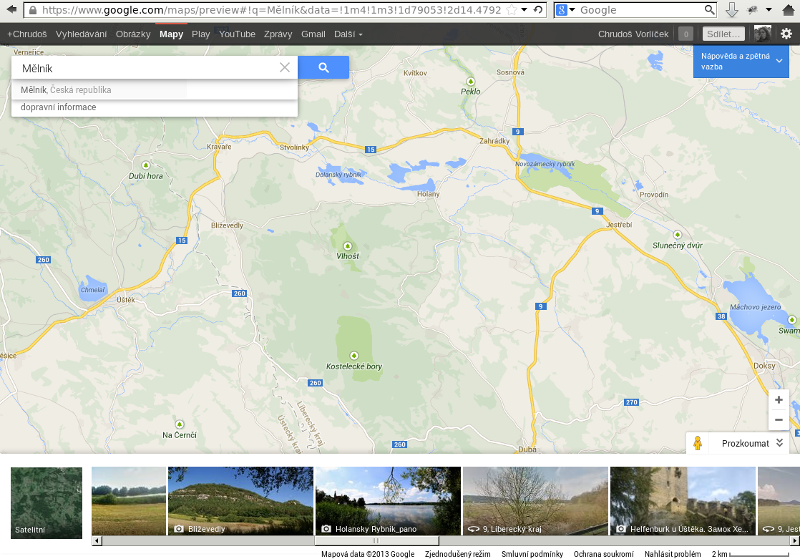
\includegraphics[width=12cm]{obrazky/googleMaps.png}
				\caption{Google Mapy s přehledem obrázků}
			\end{center}
		\end{figure}

			\begin{figure}[!h]
				\begin{center}
					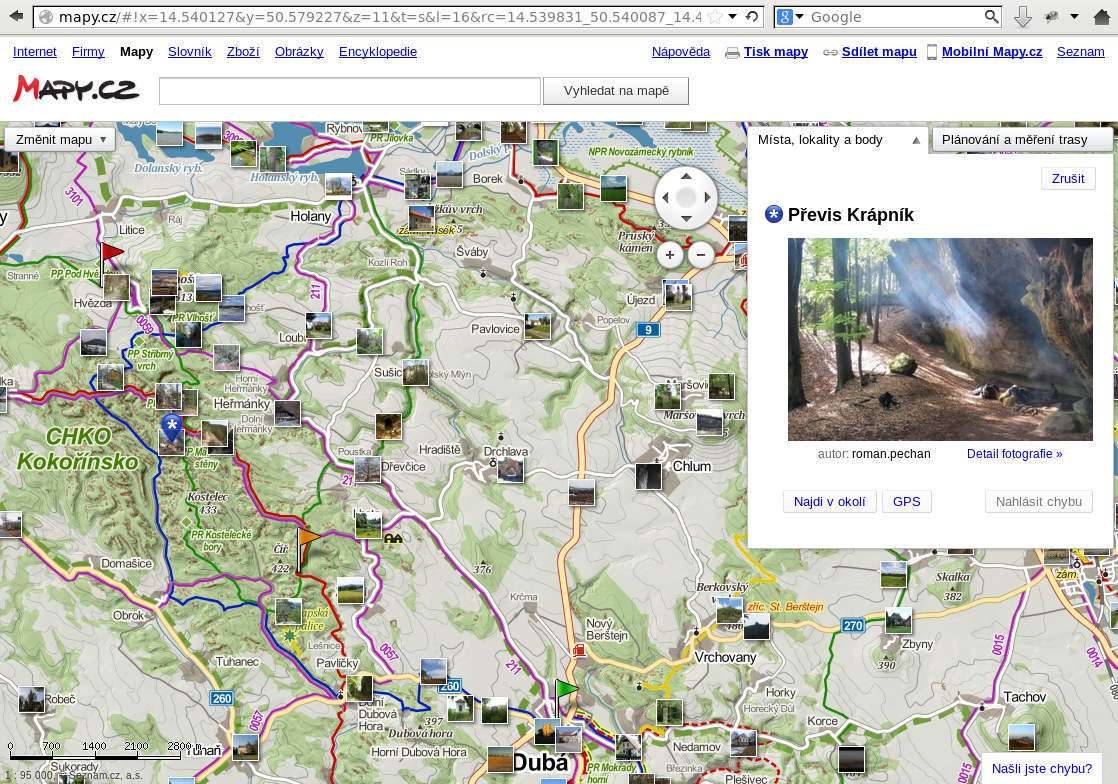
\includegraphics[width=12cm]{obrazky/mapycz.png}
					\caption{Turistická mapa na Mapy.cz}
				\end{center}
			\end{figure}

	\section{Mapy.cz}
		\url{http://mapy.cz/}
		\paragraph{} Česká mapová aplikace, která má mnoho příznivců a která je schopná konkurovat vyhledávacímu monopolu Googlu. Mapy.cz mají oproti Googlu výhodu -- zaměřují se pouze na Českou republiku. Díky tomu poskytují velké množství kvalitních mapových podkladů s velkou škálou funkcí. Od jednoduchého přidávání bodů a jejich sdílení přes vyhledávání k měřícím funkcím a vyhledávání tras. V závislosti na typu dopravního prostředku používá k vyhledávání i turistické značky a lesní cesty. Taky je možné vyhledanou cestu uložit či zobrazit její výškový profil. Mapy.cz také umožňují nahrávání fotografií a jejich komentování.

		\begin{figure}[!h]
			\begin{center}
				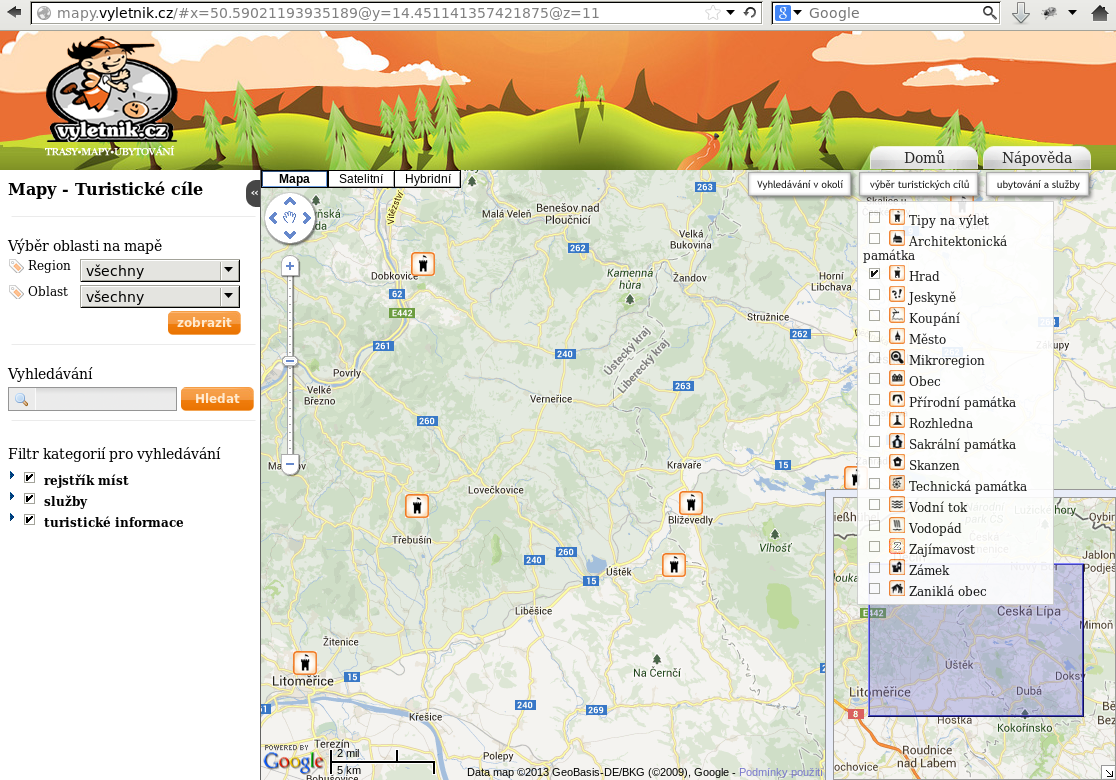
\includegraphics[width=11cm]{obrazky/vyletnik.png}
				\caption{Mapová aplikace portálu Výletník}
			\end{center}
		\end{figure}

	\section{Výletník}
		\url{http://mapy.vyletnik.cz/}
		\paragraph{} Portál Výletník poskytuje informace o turistických a cykloturistických stezkách a má i mapovou aplikaci s bodovou vrstvou možných turistických cílů, kterých je velké množství. celá aplikace je vytvořena za pomoci Google API. Díky tomu nejsou v mapě vidět turistické trasy, což mapě hodně ubírá. Na druhou stranu poskytuje možnosti vyhledat ubytování a vyhledat zájmové body v okolí. Přidanou hodnotou této aplikace je množství tipů na výlet a seznam aktuálně konaných akcí.
	
	
	\section{Waymarked Trails}
		\url{http://waymarkedtrails.org/cs/}
		\paragraph{} Aktuální přehled stezek pro turistiku, cykloturistiku a jízdy na inline bruslích je možno najít na mapě Waymarked Trails\cite{Waymarked}. Tato aplikace je vytvořena nad daty \textit{OpenStreetMap} a pokrývá celý svět. Největší množství dat je v Evropě, zbylé části světa jsou z velké části bez dat, ikdyž občas nějaká data obsahují. Nejvíce dat je poskytují vrstvy s turistickými a cykloturistickými stezkami. O poznání menší množství dat poskytují vrstvy pro horskou cyklistiku a inline bruslení.

		\begin{figure}[!h]
			\begin{center}
				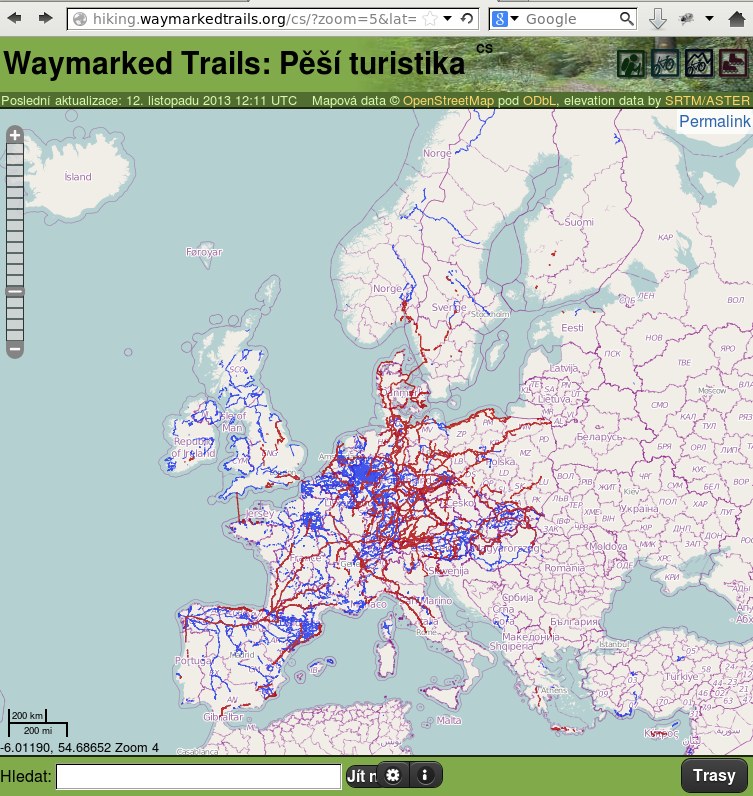
\includegraphics[width=7.5cm]{obrazky/waymarkedTrails.png}
				\caption{Hiking Map na Waymarked Trails}
			\end{center}
		\end{figure}
	
		\paragraph{} Velkou výhodou této mapy je poskytování informací o trasách a možnost jejich uložení v GPX formátu. Trasy jsou rozděleny na:
	\begin{itemize}
		 \item kontinentální -- mezinárodní trasy vedoucí přes několik států, značené prefixem E
		 \item národní -- trasy KČT
		 \item regionální -- trasy KČT
     		 \item ostatní -- naučné stezky, odbočky k hradům, zříceninám, vyhlídkám, přírodním zajímavostem apod.
	\end{itemize}
  Mapa také poskytuje možnost vyhledání místa podle názvu a vytvoření permanentního odkazu na mapový výřez. Mapa neposkytuje vyhledávání tras -- na to je potřeba použít jiná existující řešení, např. OpenRouteService (\url{http://www.openrouteservice.org/}), které kromě vyhledání trasy pro určitý typ dopravy (autem, na kole, pěšky) poskytuje i její export, výškový profil, vyhledání zájmových bodů v blízkosti.
 	\section{OpenTrackMap}
		\url{http://opentrackmap.cz/}
		\paragraph{} Posledním z výběru je český projekt OpenTrackMap Ing. Radka Bartoně z roku 2009. Motivací pro tento projekt bylo postupný nárůst užívání GPS přístrojů v turistice a nutnost map pro ně. V té době existující mapy nebylo možno použít z důvodu licenčních či technických omezení\cite{OTM}. Projekt využívá dat OpenStreetMap, která jsou uložena v PostgreSQL databázi a vykreslovány pomocí softwaru Mapnik. Aplikace poskytuje pouze možnost vykreslení turistických tras, vrstevnic a stínování terénu. V současné době mapa není aktuální.
		\begin{figure}[!h]
			\begin{center}
				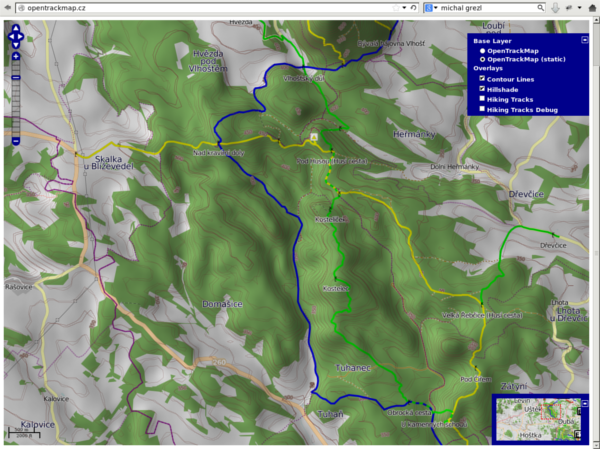
\includegraphics[width=12cm]{obrazky/otm.png}
				\caption{OpenTrackMap}
			\end{center}
		\end{figure}

%%%%%%%%%%%%%%%%%%%%%%%
%%%%% POUŽITÉ TECHNOLOGIE%%%%%
%%%%						      %%%%
%%%							  %%%
%%								     %%
%									 %
\chapter{Použité technologie}
	\paragraph{} Pro potřeby této práce byly užité technologie rozděleny na servery, které zpracovávají data, databázi a její doplňky a užité programovací jazyky. V této kapitole budou všechny postupně popsány.

%%%Servery
	\section{Servery}
		\paragraph{} Serverem rozumíme aplikaci běžící na počítači, která zpracovává dotazy a posílá odpovědi. Podle toho, jaké požadavky daný server zpracovává, mluvíme o webovém (web server), poštotovním (mail server), databázovém (database server), mapovém (map server) a jichých serverech. Protože se jedná o programy, tak je možné, aby na jednom stroji běželo velde sebe i více serverů. Pro potřeby této datové aplikace byl využit webový server Apache HTTP Server\cite{apache} a mapový server Geoserver.
		\subsection{Apache HTTP Server}
			\paragraph{} Jak už bylo řečeno v předchozím odstavci, Apache HTTP Server (častěji označován pouze jako Apache) je webový server. Jeho funkce spočívá v přijímání požadavků, jejich zpracování a odeslání odpovědi. Zpracováním se rozumí např. odeslání statické webové stránky nebo předání požadavku dalším aplikacím. Samotná komunikace je zajištěna přes hypertextový přenosový protokol (HTTP -- HyperText Transfer Protokol) Množství možných modulů značně rozšiřují možnosti samotného jádra programu. Příkladem modulu může být mod\_rewrite, který slouží k přepisování URL adresy, mod\_php rozšiřující Apache o podporu PHP nebo mod\_ssl pro šifrované spojení. Tento výčet je jen malou částí množiny.
			\paragraph{} Apache je open--source free--to--use software, což znamená, že kdokoliv ho může bezplatně užívat, prohlížet zdrojové kódy a upravovat je. Apache je také multiplatformní software s podporou všech hlavních operačních systémů. Tato strategie je výhodná a Apache je díky ní pravděpodobně nejrozšířenějším webovým serverem. Dle odhadů z června 2013 obsluhovaly servery s Apachem  54,2\% všech aktivních vebových stránek\cite{wiki-Apache}. Ikdyž je Apache vyvíjen jako open--source, jeho rychlost je srovnatelná s rychlostí výkoných komerčních serverů. 
			\paragraph{} Důvodem pro užití Apache byly přednosti vyjmenované výše -- zejména rychlost a to, že se jedná o svobodný software. Jeho nastavení se sice provádí pomocí textového editoru, to ovšem není taková překážka, protože webové stránky projektu poskytují dostatečnou dokumentaci. V případě problémů není složité dohledat řešení na internetových fórech věnovaných právě serverům.

		\subsection{Geoserver}
			\paragraph{} Stejně jako webový server zpracovává dotazy na webové stránky, mapový server zpracovává dotazy na prostorové informace. Dotaz se povětšinou skládá z řady parametrů. Většinou se jedná o zadání výřezu, seznam vrstev, v jakém formátu se mají data vrátit atd. 
			\paragraph{} Geoserver je open--source program napsaný v Javě, který umožňuje publikovat prostorová data. V současné době se jedná asi o nejlepší nekomerční řešení\cite{vorlicek}, které podporuje nejen službu WMS (Web Mapping Service), ale i WFS (Web Feature Service) a WFS-T (Web Feature Service - Transactial) a WCS (Web Coverage Service). Kromě webových služeb, poskytuje Geoserver i množství výstupních formátů. Od rastrových jpeg a png obrázkůpřes KML a PDF po GeoJSON, GML a Shapefile.
			\paragraph{} Geoserver má jednoduché uživatelské rozhraní zajištěné pomocí webové stránky. Toto rozhraní poskytuje všechny potřebné funkce pro správu uživatel-ských rolí, správu dat a jejich publikování. Pro nastavení pravidel zobrazení se užívá XML(eXtended Markup Language) schéma SLD (Styled Layer Descriptor). Tyto pravidla je možno zapsat jako SLD do textového pole nebo je lze vytvořit v externí aplikaci (například AtlasStyler SLD editor\cite{atlas} nebo Quantum GIS\cite{qgis}) a poté importovat.
			\paragraph{} Výběr Geoserveru byl dán nutností využít WFS-T službu a snahou využít pouze svobodný software. Snaha o využití WFS-T znemožnila použít UMN MapServer, protože ji nepodporuje. Oproti MapServeru má navíc výhodu uživatelského rozhraní, které MapServer postrádá -- nastavení se provádí pomocí konfiguračních souborů.

%%%Databáze
	\section{Databáze}
		\paragraph{} Většina webových aplikací potřebuje operovat s daty. Ať už se jedná o údaje o uživatelích, seznam článků či souřadnice skladů, vždy je potřeba je nějak uložit, aby se s nimi jednoduše operovalo. Jedním z možných přístupů je relační databáze. Mnoho aplikací užívá databázi MySQL, protože je rychlejší než PostgreSQL. Přestože je MySQL rychlejší a poskytuje i rozšíření pro prostorová data, je mnohem lepší využít PostgreSQL, protože poskytuje širší spektrum funkcí.
		\subsection{PostgreSQL}
			\paragraph{} PostgreSQL je open--source databázový systém. Jedná se o relační databázi, která běží na všech hlavních platformách. V PostgreSQL je podporována většina datových typů daných normou SQL:2008. Implementace SQL v PostgreSQL odpovídá standartu ANSI-SQL:2008\cite{postgresql}. Samozřejmostí je tedy podpora primárních (PRIMARY) a cizích klíčů (FOREIGN KEYS), podmínky UNIQUE a NOT NULL. Indexy mohou být uloženy v B-stromech, R-stromech, hashích nebo GiST(Generalized search tree) metodě.
			\paragraph{} PostgreSQL se dá přizpůsobit, díky čemuž existují některá rozšíření.
		\subsection{Rozšíření}
			\subsubsection{PostGIS}
				\paragraph{}
			\subsubsection{PgRouting}
				\paragraph{}

%%%Programovací jazyky
	\section{Programovací jazyky}
		\subsection{Server--side}
			\subsubsection{PHP}
				\paragraph{} Pro zpracování dynamických požadavků na serveru je potřeba použít nějaký programovací jazyk. Tyto jazyky bývají označovány jako server--side. Patří mezi ně ASP, ASP.NET, C ( při použití CGI rozhraní), Java, Perl, PHP a další. V této aplikaci je použit poslední jmenovaný jazyk. PHP\footnote{název je rekurzivní zkratka -- PHP: Hypertext Preprocessor} je určený především pro tvorbu dynamických webových aplikací, ale lze ho využít i pro tvorbu konzolových a desktopových aplikací. PHP je platformně nezávislý programovací jazyk, který lze rozšířit mnoha knihovnami. Pro tvorbu webových aplikací se PHP nejčastěji užívá se serverem Apache a databází MySQL. Tyto tři aplikace lze stáhnout v jednom balíku, který je podle platformy označován zkratkou LAMP(pro Linux) nebo WAMP(pro Windows).
				\paragraph{} Současná verze PHP je 5.5, která byla vydána k 20.6.2013. Při vývoji se užívá buď čisté PHP a nebo v podobě frameworků, které mají už naprogramované často užívané prvky. Tímto je usnadněna práce práce programátora, protože se může plně věnovat úkolu. Frameworky také zajišťují větší bezpečnost, protože úkony jako přístup do databáze jsou již ošetřeny proti chybám a programátorovi stačí zavolat potřebnou funkci. Argumentem proti frameworkům je nižší rychlost zpracování požadavků a potřeba se naučit práci s ním. Pokud se framework používá na větších nebo na více projektech, tak čas, který práce s frameworkem ušetří, je větší než doba, která je potřeba naučení se ho.

			\subsubsection{Framework Nette}
				\paragraph{}

			\subsubsection{Návrhový vzor}
				\paragraph{} Návrhovým vzorem rozumíme architekturu aplikace. Jinými slovy se jedná o určité části(vrstvy) aplikace, které zajišťují různé funkcionality. V Nette se užívá architektura MVP (Model -- View -- Presenter).
				\paragraph{Model} je označení pro vrstvu, která se stará o propojení s databází. Vkládání, změna, výpis i mazání dat jsou akce, které jsou záležitostí modelu. Model má nadefinované své funkce, kterými obsluhuje databázi. Okolí komunikuje s modelem pomocí pevně daného rozhraní. V Nette je tato vrstva implementována v knihovně Nette\\Database. Pro větší přehlednost se vytvářejí funkce, které vypisují potřebná data. Tím nedochází k pokládání dotazů ve zdrojovém kódu Presenterů.
				\paragraph{View} je vrstva, která vykresluje výsledek zadaného požadavku. V Nette se o tuto funkci starají šablony napsané latte. Latte je šablonovací systém napsaný v PHP, ovšem díky němu je psaní šablon jednodušší, přehlednější a bezpečnější než kdybychom je psali v čistém PHP.
				\paragraph{Presenter} je spojovací vrstva, která předává data z modelu do view k vykreslení a akce z view zpracovává a předává modelu. Presenter je ekvivalentem Controlleru z architektury MVC s tím rozdílem, že Controller zpracovává i některé události uživatelského rozhraní.
	\section{User--side -- JavaScript (OpenLayers vs LeafLet, jQuery)}
	\section{Grafický design -- bootstrap \cite{bootstrap}}



%%%%%%%%%%%%%%%%%%%%%%%
%%%%% 	VÝVOJ APLIKACE	   %%%%%
%%%%						      %%%%
%%%							  %%%
%%								     %%
%									 %
\chapter{Vývoj aplikace}
		\section{Databáze}
			\subsection{Datový model}
				\paragraph{} graf propojení, seznam tabulek, přehled sloupců (ne pro data OSM - spousta nadbytečných NULL hodnot) ??redukce sloupců??
			\subsection{Naplnění databáze}
				\paragraph{} Naplnění databáze se sestávalo z několika kroků. Prvním z nich bylo zajištění podpory pro PostGIS a PgRouting. Tato rozšíření budou využita v aplikaci při vyhledávání cest a zobrazování prostorových dat.
				\paragraph{}Dalším z nich bylo získání a nahrání prostorových dat. Data OSM byla stažena z  \url{http://download.geofabrik.de/europe/czech-republic.html}, kde je k dispozici vždy aktuální verze. Tato data lze importovat do databáze pomocí programu \textit{osm2pgsql}. Při vývoji na lokálním počítači vznikl problém s importem databáze. Používaný počítač neměl dostatečnou operační paměť pro jednoduchý import. Program \textit{osm2pgsql} pamatuje na starší a slabší počítače, tudíž má nastavení, která využívají přechodná úložiště v databázi a efektivněji využívají operační paměť. Databáze České republiky zabírá okolo 4 GB paměti. Vzhledem k tomu, že velká část těchto dat je nadbytečná, byla potřebná data extrahována a uložena do nové tabulky. Při této příležitosti byly vytvořeny i sloupce pro snadnější přístup k datům ve sloupci \textit{tags}. Zejména se jednalo o barvu turistické značky a její typ. Export dat a jejich úprava byly provedeny pomocí jazyka SQL. Některá data jsou ale uložena v polích. U těchto dat bylo problematičtější dostat požadovaný výsledek, ovšem dokumentace k \textit{PostgreSQL}\cite{PostgreSQL} je dobrá a na příkladech jsou uvedeny i možnosti, jak získat data z polí.
				\paragraph{} V dalším kroku bylo potřeba dovytvořit tabulky pro ukládání uživatelů, příspěvků v  diskuzi, poznámek k trasám, fotek a jiných informací. Tyto tabulky jsou neprostorové, ikdyž některé z nich se mohou mít odkazy na určité prostorové umístění.

		\section{Grafický návrh}
			\subsection{základní vzhled webové stránky - základní styl bootstrapu}
		\section{Mapové okno}
			\subsection{OpenLayers}
				\subsubsection{Zprovoznění WFS}
			\subsection{LeafLet}

		\section{Uživatelské rozhraní}
			\subsection{Přihlašování uživatelů}
				\paragraph{}K ukládání registrovaných uživatelů byla v databázi vytvořena tabulka \textit{users}. Tabulka ukládá data jak uživatelů registrovaných na stránkách, tak uživatelů přihlášených přes Facebook.
				\subsubsection{Bez Facebooku}
					\paragraph{} K příhlášení bez propojení s Facebookem je potřeba se registrovat na stránce. K tomu slouží jednoduchý formulář, kde uživatel zadá požadované informace. Formulář je opatřen i pasivním filtrem proti robotům, kteří by opakovaně vytvářeli účty a zahlcovali tak databázi. Navíc by tím získali přístup k editaci dat, což je nežádoucí. Teoreticky by mohlo dojít k masovému ukládání špatných dat do OSM. 
				\subsubsection{S Facebookem}
					\paragraph{} 
			\subsection{Dostupné funkce}
				\paragraph{}

		\section{Propojení s Facebookem}
			\subsection{Použité pluginy}
				\paragraph{} Pro propojení sociální sítě Facebook s vyvíjenou aplikací byl použit plugin pro Nette\cite{nette20login} od Jakuba Marka. Tento plugin značně usnadnil tvorbu přihlašování. Dalším pluginem, který byl použit, je FbTools\cite{FbTools} od Milana Šulce. Tento plugin poskytuje funkcionality běžně dostupné na Facebooku, např. tlačítko \textit{Líbí se mi} nebo vlákno s \textit{komentáři}.
			\subsection{Práva}
				\paragraph{} Pro správné fungování funkcionalit je potřeba si vyžádat potřebná  práva. Zde se vyskytuje problém, protože toto lze nastavit pouze při prvním přihlášení uživatele. Pozdější změny jsou možné pouze tehdy, když si uživatel odebere aplikaci a poté si ji znovu přidá s novými právy. Základní právo, které je potřeba k přihlášení je \textit{email}, které povoluje získání emailu. Pro možnost publikovat na zdi, dávat \uv{lajky} a přidávat komentáře je potřeba mít právo zveřejňovat akce nazvané \textit{publish\_actions}. Toto jsou práva, o která si aplikace říká, ale nejsou jediná. Všechna práva jsou popsána v API dokumentaci\cite{FbApiPrava}.
			\subsection{Zvežejňování na zdi}
				\paragraph{} {\Huge něco o zveřejňování a sdílení}
				\paragraph{} Bylo zjištěno, že pokud se uživatel odhlásí z aplikace, ale zůstane stále přihlášen na Facebooku, tak může zveřejňovat věci na zdi. V momentě, kdy se na počítači střídá víc lidí, může dojít k situaci, kdy jeden uživatel, který vůbec nemusí mít účet na Facebooku, bude moci publikovat statusy na zdi někoho, kdo byl na počítači před ním a zapomněl se odhlásit z Facebooku. Protože toto je nežádoucí jev, byly proti němu učiněna opatření v podobě skrytí tlačítka, které sdílení vyvolávás. Tlačítko se zobrazí jen v případě, že má uživatel u svého účtu uloženo v databázi \textit{fbuid}, což je označení pro pole v tabulce \textit{user}, ve kterém je uloženo uživatelská indentifikace obdržená z Facebooku.
		
		\section{Editace dat}
				\paragraph{} Pro umožnění editace dat existovala dvě možná řešení. První řešení zahrnuje vytvoření vlastního rozhraní, druhé pak použití existujícího řešení a připojení k stávající aplikaci. U druhého řešení byla od začátku zvažována možnost použití HTML5 editoru \textit{iD}. Protože obě řešení mají své výhody a nevýhody, budou zde vypsány obě.
			\subsection{Tvorba vlastního rozhraní}
				\paragraph{} První řešení, jak už bylo řečeno, zahrnuje vytvoření jednoduchého rozhraní. Prvky by se editovaly a  ukládaly do databáze projektu a v určitých intervalech by byl prováděn import těchto dat do OpenStreetMap. Výhoda této metody spočívá v tom, že data by mohla být kontrolována, zda jsou fakticky správně, aby nedocházelo k znehodnocení dat OpenStreetMap. Také by bylo možno tuto funkci implementovat s minimálními změnami pro přidávání vlastních cest. Na druhou stranu by toto řešení znamenalo množství programování, protože by bylo potřeba zajistit nástroj pro import do OpenStreetMap, popřípadně data importovat ručně. V začátcích by to pravděpodobně nebyl problém, ovšem po překročení určitého počtu editací by se mohl stát ruční import nemožným nebo alespoň velice náročným na čas.
				\paragraph{} Protože zde nedochází k odesílání dat na jiný server, byl tento přístup zvolen pro přidávání vlastních cest.
			\subsection{Editor iD} 
				\paragraph{} Kvůli výše vyjmenovaným nevýhodám bylo rozhodnuto, že nejprve bude prozkoumána možnost připojení HTML5 editoru \textit{iD}, který byl vytvořen pro editaci dat OpenStreetMap. Po prozkoumání zdrojových kódů editoru bylo zjištěno, že aplikace může být připojena pomocí protokolu \textit{oAuth}. Aby aplikace nepoužívala osobní účet na OpenStreetMap, byl vytvořen speciální účet, pod kterým aplikace byla registrována. 
				\paragraph{}{\Large Byla snaha umožnit uživatelům s účtem na OpenStreetMap, aby mohli editovat data pod svým účtem. Zatím tato funkcionalita zprovozněna není.}
				\paragraph{} Editor iD má i určité nevýody. Například poskytuje více funkcionalit než je potřeba a komplexnost editoru činí modifikaci zdrojového kódu časově náročnou. Pro vytvářenou aplikaci je nadbytečná možnost editace budov. V momentě, kdy by nebyla povolena editace plošných prvků (polygonů), probíhalo by načítání dat z OpenStreetMap rychleji. 
		\section{Trasy a fotky}
			\paragraph{}

		\section{Testování}


%%%%%%%%%%%%%%%%%%%%%%%
%%%%% 		ZÁVĚR	  	   %%%%%
%%%%						      %%%%
%%%							  %%%
%%								     %%
%									 %
	\chapter{Zhodnocení}
		\paragraph{}

%%Užitá literatura
\newpage
\addcontentsline{toc}{chapter}{Reference}
\begin{thebibliography}{50}
	\bibitem{bootstrap}Bootstrap. [cit. 21.10.2013] Dostupné z: \url{http://getbootstrap.com}.
	\bibitem{nette20login}MAREK, Jakub: Přihlašování v Nette Frameworku. [cit. 21.10.2013]. Dostupné z: \url{http://github.com/janmarek/nette20login}
	\bibitem{FbTools} ŠULC, Milan: FbTools. [cit. 21.10.2013]. Dostupné z: \url{http://addons.nette.org/cs/fb-tools}.
	\bibitem{FbApiPrava} Facebook developers - Login Reference. [cit. 21.10.2013]. Dostupné z: \url{https://developers.facebook.com/docs/reference/login/#permissions}.
	\bibitem{Leaflet}	Leaflet - A JavaScript Library for Mobile-Friendly Maps. [cit. 29.10.2013]. Dostupné z: \url{http://leafletjs.com/}
	\bibitem{PostgreSQL} PostgreSQL: The world's most advanced open source database. [cit. 8.11.2013]. Dostupné z: \url{http://www.postgresql.org/}.
	\bibitem{Waymarked} Waymarked Trails.  [cit. 12.11.2013] . Dostupné z: \url{http://www.waymarkedtrails.org/cs/}
	\bibitem{OTM} BARTOŇ, Radek. Custom OpenStreetMap Rendering: OpenTrackMap Experience. In: [online]. 2009. vyd. [cit. 2013-11-12]. Dostupné z: \url{http://geoinformatics.fsv.cvut.cz/gwiki/Custom_OpenStreetMap_Rendering_-_OpenTrackMap_Experience}
	\bibitem{apache}The Apache Software Foundation: Apache - HTTP Server project. [cit. 12.11.2013]. Dostupné z: \url{http://httpd.apache.org/}
	\bibitem{wiki-Apache}Wikipedia:Appache HTTP Server. [cit. 12.11.2013]. Dostupné z: \url{http://en.wikipedia.org/wiki/Apache_HTTP_Server}
	\bibitem{geoserver}Geoserver. [cit. 13.11.2013]. Dostupné z: \url{http://geoserver.org/display/GEOS/Welcome}
	\bibitem{vorlicek}VORLÍČEK, Chrudoš: Geoportály a mapové servery v České republice, bakalářská práce. Praha: České vysoké učení technické v Praze, 2012.
	\bibitem{atlas}GeoPublishing: AtlasStyler SLD editor. [cit. 13.11.2013]. Dostupné z: \url{http://en.geopublishing.org/AtlasStyler}
	\bibitem{qgis}QGIS. [cit. 13.11.2013]. Dostupné z: \url{http://www.qgis.org/en/site/}
	\bibitem{postgresql} PostgreSQL. [cit. 13.11.2013]. Dostupné z: \url{http://www.postgresql.org/}.
\end{thebibliography}

\end{document}